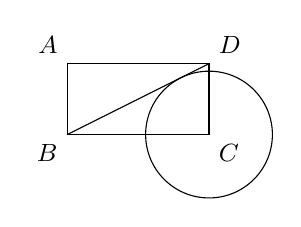
\begin{tikzpicture}[scale=.90, every node/.style={font=\small}]
  \coordinate (A) at (0,1); \coordinate (B) at (0,0);
  \coordinate (C) at (2,0); \coordinate (D) at (2,1);
  \draw (A)--(B)--(C)--(D)--cycle;
  \draw (B)--(D);
  \draw (C) circle (.8944);
  \node[above left] at (A) {$A$};
  \node[below left] at (B) {$B$};
  \node[below right] at (C) {$C$};
  \node[above right] at (D) {$D$};
\end{tikzpicture}
